\documentclass[11pt,a4paper]{article}

% Langue
\usepackage[french]{babel}
\usepackage[utf8]{inputenc}
\usepackage[T1]{fontenc}

% Mise en page
\usepackage[scale=0.7]{geometry}
% Pied de page
\usepackage{fancyhdr}
\pagestyle{fancy}
\renewcommand{\headrulewidth}{0pt}
\setlength{\headheight}{13.6pt}
% Interligne après les paragraphes
\setlength{\parskip}{5pt}

% Images
\usepackage{graphicx}
\usepackage{subcaption}
\usepackage{wrapfig}

% Rond plutôt que des tirets dans les listes
\renewcommand{\Frlabelitemi}{\textbullet}

% Bibliographie
\bibliographystyle{plain}
\usepackage{url}% Used for printing URL

\begin{document}

\newcommand{\HRule}{\rule{\linewidth}{0.5mm}}

\begin{titlepage}
\begin{center}


\includegraphics[width=0.5\textwidth]{polytech}~\\[1cm]

\textsc{\LARGE EISD}\\[1.5cm]

\textsc{\Large Extraction d'information et Système de dialogue}\\[0.5cm]

% Title
\HRule \\[0.4cm]
{ \huge \bfseries Création d'un système de dialogue complet\\ [0.4cm] }
\HRule \\[1.5cm]

% Author and supervisor
\begin{minipage}{0.4\textwidth}
\begin{flushleft} \large
\emph{Auteurs:}\\
Romain \textsc{Jayez}\\
Guillaume \textsc{Monnet}
\end{flushleft}
\end{minipage}
\begin{minipage}{0.4\textwidth}
\begin{flushright} \large
\emph{} \\
Steven \textsc{Nabbs}\\
Luc \textsc{Poncet}
\end{flushright}
\end{minipage}

\vfill

% Bottom of the page
{\large \today}

\end{center}
\end{titlepage}


\rhead{EISD - Rapport}
\lfoot{
\includegraphics[scale=0.3]{polytech.jpg}}
\rfoot{JAYEZ - MONNET \\ NABBS - PONCET}

\tableofcontents

\clearpage

\section{Introduction}
%Schema du systéme ?

Le but du projet est de créer un système permettant d'engager un dialogue question-réponse avec un utilisateur. Le système répond en puisant les informations dans une base de données. Cette base à été préalablement remplis grâce à des informations extraites depuis différents éléments comme des texte, tableaux et ceci provenant de toute sources disponibles. 
La circulation des données est illustrée par la figure \ref{fig:schema} en dessous.

\begin{figure}[!htb]
	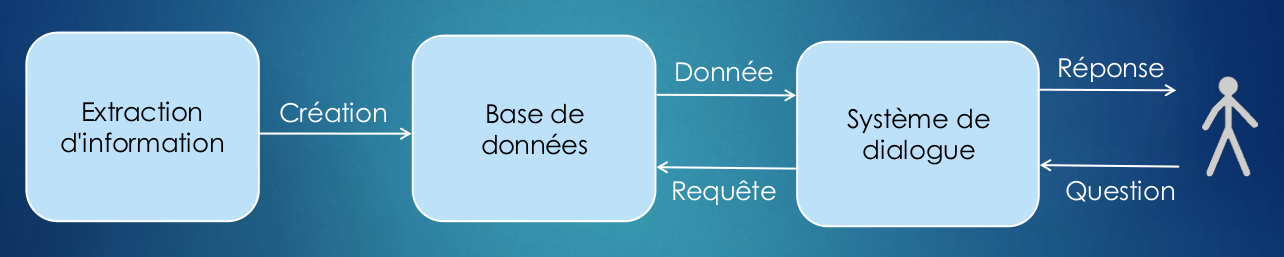
\includegraphics[width=\textwidth]{schemaSysteme.png}
	\caption{Schèma simplifié du fonctionnement de système}
	\label{fig:schema}
\end{figure}

Des systèmes équivalent de grandes ampleurs sont déjà utilisés tous les jours. Pour ce projet, il est demandé de réaliser un version minimaliste avec des informations concentrés sur un seul sujet.

Il existe plusieurs manière de récupérer et remplir une base de données, les principales sont de récupérer directement les informations depuis un tableau, c'est la manière la plus rapide, la plus simple, et on obtient une grande masse de données. Ensuite extraire l'information depuis des textes, pour cela il faut établir des listes de règles et des expression régulière pour récupérer l'information. Cette méthode est donc plus compliqué à mettre en place, mais cela permets toujours d'automatiser la récupération de l'information. Ensuite quand les informations sont ne sont pas récupérable par les méthodes précédente, il est plus rentable d'ajouter manuellement une information dans la base de données que de créer une règle spécifique.
Dans le projet on utilise la méthode d'extraction d'information dans les textes pour remplir de la base. Cela nous permets d'être confronté aux problèmes que pose la rédaction des règles.

Deux sujets était proposés, le premier, des descriptions provenant du site Wikipédia d'un grand nombre de pays. Le second, des recettes et commentaires issues du site Marmiton. Nous avons choisis les descriptions des pays pour la propreté de rédaction des textes.

Le projet est réaliser en langage lua, langage de script léger et performant. On utilise un programme nommé dark qui est un outils de développement pour la création des règles. Celle-ci s'utilise de la même manière que des expressions régulières. L'outil permet également l'application de tag dans les textes et une sérialisation de tableau pour remplir la base de données faite en lua. 


\clearpage

\section{Extraction d'information}

\subsection{Composition de la base de données}

Pour démarrer, nous avons regardé une certaine quantité de description sur les pays et nous avons repéré les informations récurrente dans chaque fichier. Avec ceci nous avons crée la base fictive contenant chaque type d'information que l'on aimerait récupérer.

Choix initial des informations à récupérer :
\begin{itemize}
	\item Capitales
	\item Pays Frontaliers
	\item Monnaie
	\item Continent
	\item Religions
	\item Population
	\item Régime
	\item Superficie
	\item Position (GPS, etc.)
\end{itemize}

L'information Position devait contenir une position GPS, ou tout autre élément permettant de situer le pays. Or la position GPS n'est pas présente dans les différents textes et la position est déjà donnée grâce aux informations Continent et Pays Frontaliers. Donc nous avons retirer l'information Position de notre base de données.


\subsection{Les problèmes rencontrés}
Au cours de ce projet, plusieurs problèmes ont été rencontré quant à l'extraction des informations.
En effet, les informations contenus dans les différents textes ne sont pas formatés selon un schéma particulier.
Ainsi, une même information (telle que la capitale d'un pays) pourra être donné de nombreuses façon différentes.
Dès lors, il devient difficile de créer des règles de pattern capable de récupérer l'ensemble des informations contenues dans les textes.

Autre problème découlant du précédent : la création des règles de pattern a été réalise de manière plutôt "empirique".
Après lecture de quelques pays, une règle générale est créé.
Cependant, des versions "alternatives" de cette règles doivent être peu à peu créé pour couvrir plus d'informations.
Ainsi, certaines règles pouvaient rapidement devenir complexes.

Toujours dans la création des règles de pattern, nous avons rencontrés une contrainte lié directement à l'outil de travail : dark.
En effet, si celui-ci reconnaissait généralement assez bien les types des mots, il arrivait dans certains cas qu'un mot soit reconnu comme appartenant à un autre type (par exemple un nom propre reconnu comme étant un adjectif), empêchant ainsi le bon fonctionnement des règles préalablement écrites et ne permettant pas la bonne récupération de l'information.

La ponctuation a également posé problème dans sa gestion.
Si au départ des espaces étaient insérés autour de chaque élément de ponctuation, il s'est rapidement avéré qu'un tel choix engendrait des difficultés supplémentaires pour la reconnaissance des mots composés (par exemple, "antigua-et-barbuda" devenait "antigua - et - barbuda" et n'était donc plus reconnu comme un pays).
Il a été donc décidé de restreindre les éléments de ponctuations à séparer par des espaces.

Par rapport à la génération de la base de donnée, il nous a été dans un premier temps difficile de récupérer les informations tagués dans les textes.
Une première tentative lourde et approximative a été de considérer les textes traités comme étant des fichiers type XML.
En utilisant une librairie lua existante, il était ainsi possible de récupérer le contenu des balises.
Cette méthode n'était cependant pas optimale et a rapidement été remplacer par l'utilisation de fonction de récupération direct de tag fournies ainsi que de variantes créés lorsque le besoin se présentait.

Enfin, la dernière difficulté rencontrée découle directement d'un mauvais choix de méthode de travail.
En effet, nous avons eu tendance à plutôt nous concentrer sur une seule information à la fois et créer le plus de règle possible pour essayer de récupérer cette information dans tous les pays.
Plutôt que de consacrer beaucoup de temps à la création de règles spécifiques qui ne vont récupérer l'information que dans 2 ou 3 pays supplémentaires, nous aurions du passer aux informations suivantes (quitte à y revenir une fois que toutes les informations était récupérées dans des proportions correctes).

\subsection{La couverture d'information de la base}
Nous avons réaliser un script permettant de calculer le rapport d'information présente dans la base de données par rapport au nombre total de pays.

Voici les résultats (arrondi au \%) après avoir effectué les dernières modifications sur nos règles :
% bla bla completage
\begin{itemize}
	\item Langue 		  : 22\%
	\item Continent 	  : 84\%
	\item Capitale 		  : 38\%
	\item Pays Frontalier : 43\%
	\item Superficie	  : 21\%
	\item Population 	  : 38\%
	\item Régime 		  : 9\%
	\item Religion		  : 12\%
	\item Monnaie		  : 22\%
\end{itemize}

  


\subsection{Améliorations possibles}
Vérifications de la qualité des informations dans la base de données :
Par exemple, la liste des pays frontalier d'un pays X, on peut vérifier que chaque pays contenu dans la liste, a bien le pays X comme pays frontalier.

\clearpage

\section{Système de dialogue}

\subsection{Choix effectues}

\subsubsection{Les Tags} 

Le but de la reconnaissance d’informations est de taguer les informations essentielles dans la question, à savoir le contexte et le sujet. Le contexte ici étant le pays, et le sujet étant les informations importantes le concernant. Ces informations sont les suivantes :
\begin{itemize}
	\item Capitale
	\item Pays frontaliers
	\item Monnaie
	\item Continent
	\item Religions
	\item Population
	\item Régime
	\item Superficie
\end{itemize}

Nous avons donc taguer ces informations et nous les avons reliées à des mots à connotation proche pour identifier le sujet d'une question poser par l'utilisateur même s'il choisit de s'exprimer différemment. Par exemple, lorsqu'un utilisateur interroge le programme sur les religions d'un pays, il peut employer les termes "culte", "croyance", "dogme", "confession", "superstition", "foi" ou "religion".

\subsubsection{Stockage et recupération de données}

Nous avons choisi de stocker la réponse aux informations dans la base de données de la sorte :
France {
	monnaie = ‘’,
	capitale = ‘Paris’,
	religions = {},
	pays\_frontaliers = { Espagne, Allemagne, Suisse }
}
Soit un champ est vide, soit il contient une valeur, ou soit il contient un tableau de valeurs (qui peut être vide également). 

Ainsi, lors d'un parcours de la base, on utilise la méthode for k,v in ipairs, (k étant la clé et v la valeur) et on teste si ces valeurs sont nuls, si elles constituent une valeur unique, ou si ce sont des sous tableaux de valeurs. 

\subsubsection{Parsage des données}

\paragraph{}Nous avons décidé de ne pas prendre en compte les majuscules lors de la définition d'un nom de pays pour une question car si l'utilisateur ajoute plusieurs majuscule à un nom de pays ou à un élément clé sujet de la question comme "FranCE" ou "DEVise", on aurait eu à faire un traitement supplémentaire pour les identifier. Ainsi, les données sont stockées sans majuscule en base de données et au moment de la saisie d'une question, les données saisies sont immédiatement réduites en minuscule et on y enlève les éléments de ponctuation n'apparaissant pas comme pertinents à l'exception du point d'interrogation. 
\paragraph{}Nous avons choisi de parser la question et de nous arrêter à la lecture du point d’exclamation. Tout ce qui suit le ‘ ?’ n’est pas pris en compte. Cela nous permet d’éviter de devoir traiter plusieurs questions en même temps. Si l’utilisateur ne rentre pas de point d’exclamation la question n’est pas reconnue comme telle et nous n’y donnons donc pas suite.

\subsubsection{Affichage syntaxique dans un français correct}

\paragraph{}Une difficulté dans un tel projet est d'associer un article à un nom de pays, par exemple "La France" ou "Le Canada". Dans ces exemples il est difficile de concevoir une machine capable de détecter si le programme doit répondre au féminin, au masculin ou même au pluriel. De même en répondant "de la France" ou "du Canada". Pour remédier à ce problème nous avons choisi de répondre par "le pays nommé France" ou "du pays nommé Canada". Cela permet de lever l'ambiguïté tout en restant dans un français correct. 
\paragraph{}Néanmoins, pour les sujets, un réel traitement est effectué. C'est-à-dire que nous testons conditionnellement le type de sujet (monnaie, continent, pays frontaliers) et le type de question (singulier, pluriel). En fonction du nombre de réponse on aura un affichage adapté. Soit, si on demande les religions en France, la réponse sera du type "les religions du pays nommé France sont <Liste des religions en France>". 
\paragraph{}Aussi lorsque l'utilisateur interroge directement les données en base, le nombre de réponses est affiché et un choix lui est proposé quant à sa volonté d'afficher le résultat ou non. Cela lui permet d'éviter de surcharger la zone graphique si jamais le résultat est trop élevé ou si l'utilisateur a réalisé une erreur de frappe.

\subsubsection{Historique des questions/réponses}
Nous avons pensé à garder en mémoire dans une liste toutes les informations concernant la question posée précédemment par l'utilisateur, et la réponse fournie par le programme. Ainsi, nous avons testé si la question contient bien un sujet, un contexte, ou si elle portait sur une multitude d'éléments, ou alors sur la base directement. 
\paragraph{}De ce fait, l'utilisateur peut poser une question avec un ou plusieurs sujet(s) concernant un ou plusieurs pays. Puis poser une question concernant un ou plusieurs sujets et celle-ci sera alors associée au(x) pays précédemment stocké. L'utilisateur peut même demander quels sont les pays frontaliers d'un pays et réutiliser la réponse comme un nouveau contexte à la question suivante.
\paragraph{}D'autre part, les questions de l'utilisateur doivent rester cohérentes. En effet, si jamais il interroge la base sans aucun sujet ou avec un sujet et des contextes multiples, le programme ne sera pas en mesure de lui répondre.

\subsubsection{Jointure de données}
\paragraph{}Nous avons décidé d'implémenter un tag jointure comprenant les termes "commun", "similaire", "semblable", "identique", et "entre". Ce tag permet de renvoyer la réponse à des sujets que plusieurs pays possèdent en commun. Cela permet à l'utilisateur d'effectuer des comparaisons entre pays dans la base.

\subsection{Fonctionnalités désirées}

\paragraph{}Nous avons pensé à poser une question du type : «  Quels sont tous les pays dans la base de données qui possèdent l’euro ?». Pour répondre à cette question nous aurions pu parcourir la base jusqu'à atteindre le mot « euro » une première fois puis  récupérer le tag « monnaie » associé à ce mot. Enfin nous aurions récupéré tous les pays dont le tag « monnaie » contiendrait « euro ». Mais finalement, nous avons conclu que cela ne pourrait marcher que pour une petite base de données donc nous avons choisi de ne pas implémenter ce type de réponse. 
\paragraph{}Nous aurions également aimé pouvoir implémenter une solution de traitement des mots à connotation proche pour pouvoir regrouper les langues, les religions et ne conserver que leur base. Par exemple, "islam" et "islamisme" sont tous les 2 en base de données mais ne concernent qu'une religion.

\subsection{Les questions types}

\textbf{Attention à toujours terminer une question par un point d'exclamation!}


Récupérer le sujet/thème de la question (capitale, monnaie, pays voisins, religion,) et récupérer le contexte/pays sur lequel la question porte. \\
\textit{« Quelle est la capitale de la France ? » }

Prendre en compte le fait qu’il puisse y avoir plusieurs sujets pour une question. \\
\textit{« Quelles sont les capitales de l’Afrique du Sud et sa devise ? »}

Prendre en compte le fait qu’il puisse y avoir plusieurs contextes pour une question. \\
\textit{« Quelle est la capitale de la France et celles de l’Afrique du Sud ? »}

Gérer l’historique pour un ou plusieurs contextes. \\
\textit{« Quelle est la capitale de l’Espagne et de la France ? »\\
	« Et leur monnaie ? »}

Gérer l’historique pour un ou plusieurs sujets. \\
\textit{« Quelle est la devise de la Belgique et ses religions ? » \\
	« Et pour la France ? »}

Ajout d’une table de jointure pour trouver si 2 pays ont des contextes en commun (ajout d’un tag sur les mots en commun). Renvoie tous les pays frontaliers en commun entre 2 pays : \\
\textit{« Quels sont les pays voisins en commun entre la France et l’Autriche ? »}

Renvoie tous les pays frontaliers en commun entre les 3 pays et renvoie ceux en commun entre 2 pays deux à deux avec un pourcentage d’intersection : \\
\textit{« Quels sont les pays voisins en commun entre la France et l’Autriche et l’Espagne ? »}

Interrogation sur un ou plusieurs pays dans base renvoie de façon structurée toutes les informations le(s) concernant \\
\textit{« Quelles sont les données en base que tu possèdes sur la France et l’Espagne ? »}

Interrogation sur un ou plusieurs sujets dans la base de données renvoie toutes les informations, sans doublons, disponibles et présentes pour chaque pays.
\textit{« Quelles sont les devises et les religions présentes en base ? »}


\section{Compilation et éxecution du projet}
Pour lancer le projet, il faut d'abord compiler l'outils dark :
Dans le dossier ou se situe le makefile de dark, il faut lancer la commande make.
Ensuite pour la création de la base de données, il faut lancer la commande suivante dans le dossier du projet :
lua creationBdd.lua
Enfin pour lancer le système de dialogue, il suffit de lancer la commande :
./dark dialogue.lua

\section{Conclusion}

Ce projet nous a permis d'appréhender le langage Lua. Ce langage se révèle être capable de faire des scripts léger et puissant. Il est justement apprécié dans le milieu professionnel pour ses qualités, et même très présent dans le milieu du jeu vidéo. L'apprentissage de ce langage pourra se montrer utile par la suite.

\end{document}
